\documentclass[border=10pt]{standalone}
\usepackage{tikz}
\usetikzlibrary{shapes,backgrounds,calc,patterns,trees}

\begin{document}
	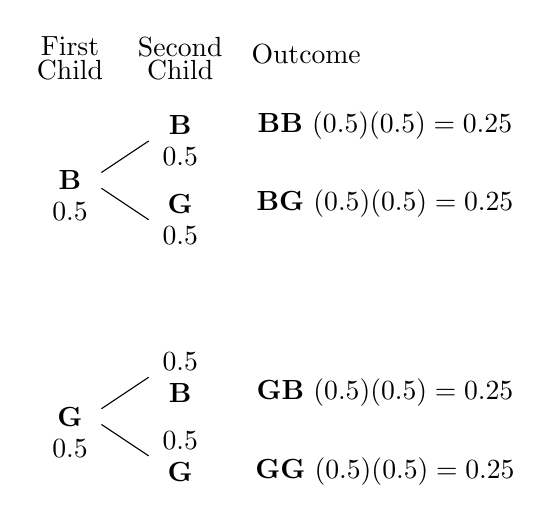
\begin{tikzpicture}
		\node at (0,3.2) {First};
		\node at (0,2.9) {Child};
		
		
		\node at (1.4,3.2) {Second};
		\node at (1.4,2.9) {Child};
		
		
		\node at (3, 3.1) {Outcome};
		
		\node [align=left] at (4,2.2) {\textbf{BB} \((0.5)(0.5)=0.25\)};
		
		\node [align=left] at (4,1.2) {\textbf{BG} \((0.5)(0.5)=0.25\)};
				
		\node [align=left] at (4,-1.2) {\textbf{GB} \((0.5)(0.5)=0.25\)};
						
		\node [align=left] at (4,-2.2) {\textbf{GG} \((0.5)(0.5)=0.25\)};
								
								
	
		
		\node at (0,1.5) {\textbf{B}};
		\node at (0,1.1) {\(0.5\)};
		
		\draw (.4,1.6) -- (1,2);
		\draw (.4,1.4) -- (1,1);
		
			\node at (1.4,2.2) {\textbf{B}};
			\node at (1.4,1.8) {\(0.5\)};
		
			\node at (1.4,1.2) {\textbf{G}};
			\node at (1.4,.8) {\(0.5\)};
		
		
		
		\node at (0,-1.5) {\textbf{G}};
		\node at (0,-1.9) {\(0.5\)};
		
				\draw (.4,-1.6) -- (1,-2);
				\draw (.4,-1.4) -- (1,-1);
		
	
				\node at (1.4,-1.2) {\textbf{B}};
				\node at (1.4,-.8) {\(0.5\)};
	
				\node at (1.4,-2.2) {\textbf{G}};
				\node at (1.4,-1.8) {\(0.5\)};
	
	\end{tikzpicture}
\end{document}

